\documentclass[
        a4paper,     % Format A4
        titlepage,   % mit Titelseite
        twoside,     % zweiseitig
        parskip      % mit Durchschuss
                                 % (= Abstand zwischen Absätzen, statt Einrückung)
        ]{scrartcl} % KOMA-Script Grundklasse     texdoc scrguide

\usepackage{ngerman}              % Deutsche Sprache, neue RS   texdoc germdoc (?)
\usepackage[T1]{fontenc}          % Schriftkodierung mit Umlauten
\usepackage{textcomp,amsmath}     % Mathezeichen etc.
\usepackage{graphicx}             % Graphiken einbinden

%%% my own packages %%%
\usepackage{url}
\usepackage{xcolor}
\definecolor{darkgreen}{RGB}{0,120,0}
\usepackage{nicefrac}

% bibtex
\bibliographystyle{plaindin}      % BibTeX Styles nach Norm DIN 1505

\titlehead{

\includegraphics{hpi_logo_cmyk_wb_sl2}
} \subject{Master's Thesis}
\title{Scanpath Comparison for Visual Search Analysis}
\author{Markus Hinsche\\{\small{\url{markus.hinsche@student.hpi.uni-potsdam.de}}}}
\date{Submitted: \today}
\publishers{Supervision: Dr. Gjergji Kasneci}

\pagestyle{headings}    % Seitenstil mit Kapitelüberschriften in der Kopfzeile


\begin{document}

  \maketitle    %  Titelseite erzeugen


  \cleardoublepage % neue Doppelseite



  % Und: Text \dots
  \section{Einleitung}

%    \cite{vossen94datenmodelle}


    \section{extended HMM}



$
v_i \in \left\{ {0\%-50,50\%-90\%,90\%-100\%} \right\}
$

priors for $v_i$ are found by selecting random sequences (with replacement). Here we take the relative number that fall in a specific range.

$
P(v_i=0\%-50\%) = \frac{\#0\%-50\%}{\#total}
$

analogously for the other ranges. 


$
x_i \in \left\{ { Fixation,Saccade} \right\}
$

$
angles = \left\{ {0\,^{\circ}-30\,^{\circ}, 30\,^{\circ}-60\,^{\circ}, 60\,^{\circ}-90\,^{\circ}} \right\}
$

$
length = \left\{ {short, long} \right\}
$

$
area = \left\{ {middle, upper right, upper left, lower left, lower right} \right\}
$


$
y_i \in \left\{ { abc | a\in angles, b\in length, c\in area} \right\}
$

% extended HMM
\begin{figure}[h]
    \centering
    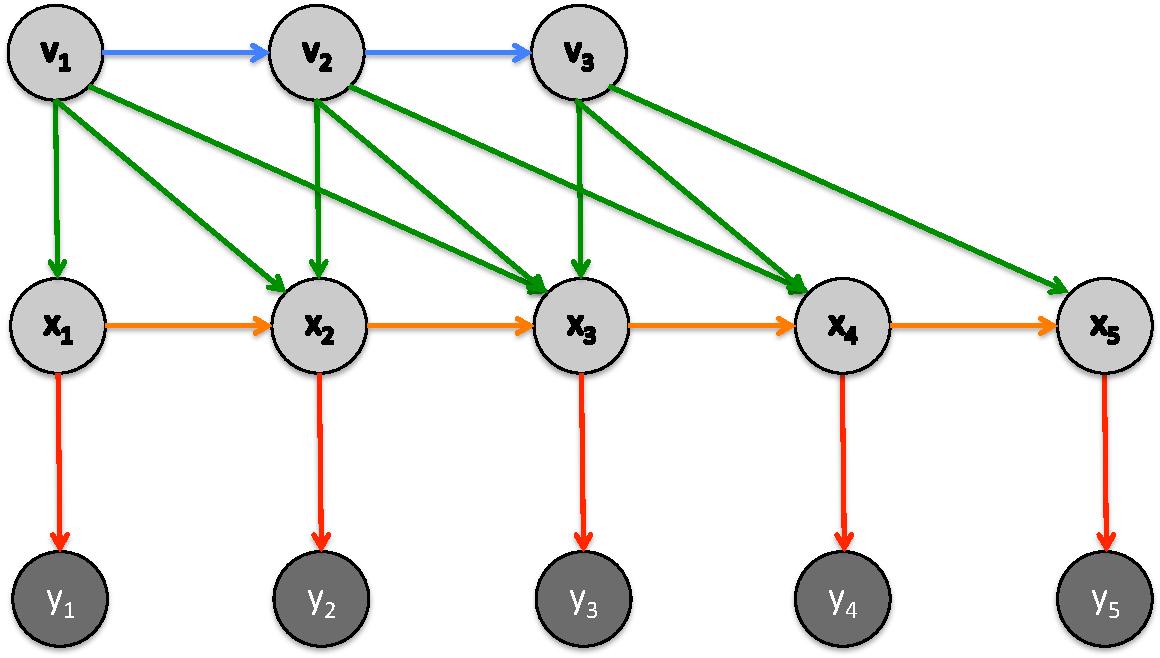
\includegraphics[width=0.6\columnwidth]{graphics/extendedHMM.pdf}
    \caption{\label{fig:extendedHMM} Model of the extendet HMM. }
\end{figure}



\color{blue}
$
A_{v_i\rightarrow v_j} =
 \begin{pmatrix}
  \nicefrac{1}{k}  & \nicefrac{1}{k} & \cdots & \nicefrac{1}{k} \\
  \nicefrac{1}{k} & \nicefrac{1}{k} & \cdots & \nicefrac{1}{k} \\
  \vdots  & \vdots  & \ddots & \vdots  \\
  \nicefrac{1}{k} & \nicefrac{1}{k} & \cdots & \nicefrac{1}{k}
 \end{pmatrix}
$


\color{darkgreen}
relative number of sequences


$ 
A_{v_i\rightarrow x_j} = = \bordermatrix{
                  ~        & Fixation & Saccade \cr
                   0\%-50\%  & a_{1,F}   & a_{1,F} \cr
                  50\%-90\%  & a_{2,F}   & a_{2,S} \cr
                  90\%-100\% & a_{3,F}   & a_{3,S} \cr}
$


\color{orange}
relative occurrence to go from state $x_i$ to state $x_j$ (according to the data). 
Use Smoothing!


$ 
A_{x_i\rightarrow x_j} = \bordermatrix{
                  ~        & Fixation & Saccade \cr
                  Fixation & a_{F,F}   & a_{S,F} \cr
                  Saccade  & a_{S,F}   & a_{S,S} \cr}
$

\color{red}
when I am in a state $x_i$, how often do I see a certain feature

%$
%A_{x_i\rightarrow y_j} =
% \begin{pmatrix}
%  a_{1,1} & a_{1,2} & \cdots & a_{1,n} \\
%  a_{2,1} & a_{2,2} & \cdots & a_{2,n} 
% \end{pmatrix}
%$
 
$ 
M_{x_i\rightarrow y_j} = \bordermatrix{
                  ~        & aA0 & aA1 & ... & bB5 \cr
                  Fixation & a_{F, aA0}   & a_{F, aA1}   & ... & a_{F, bB4} \cr
                  Saccade  & a_{S, aA0}   & a_{S, aA1}   & ... & a_{S, bB4} \cr}
$

\color{black}


    % Inhaltsverzeichnis
    \clearpage % auf neuer Seite
    \bibliography{abbreviations, referenzen}

\end{document}
